\begin{frame}{Proof Systems}

    \begin{block}{Proof system (for $\UNSAT$) [Cook, Reckhow 79]}
        Poly-time algorithm $\Pi\colon \{0, 1\}^* \times \{0, 1\}^* \rightarrow \{0, 1\}$:
        \begin{itemize}
            \item (completeness) $\varphi \in \UNSAT \Rightarrow \exists w ~ \Pi(\varphi, w) = 1$;
            \item (soundness) $\exists w ~ \Pi(\varphi, w) = 1 \Rightarrow \varphi \in \UNSAT$.
        \end{itemize}
    \end{block}

    \deftext{Resolution}: proof of $\varphi \coloneqq \bigwedge\limits_{i} C_i$ is a sequence of clauses
    $(D_1, D_2, D_3, \dots, D_{\ell})$:
    \pause
    
    \begin{minipage}{0.3\linewidth}
        \begin{itemize}
            \item $D_i \in \{C_i\}$;
                \pause
            \item $\frac{A \lor x ~~~~~ B \lor \bar{x}}{A \lor B}$, $D_i \coloneqq A \lor B$;
                \pause
            \item $D_{\ell} = \emptyset$.
        \end{itemize}
    \end{minipage}
    \pause
    \begin{minipage}{0.68\linewidth}
        \centering
        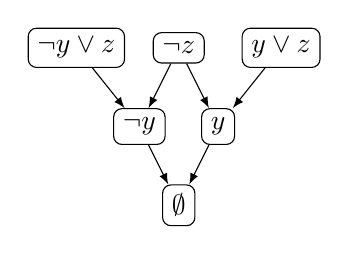
\begin{tikzpicture}[>=latex]
    \node[rectangle, rounded corners = 3pt, draw] (a) at (-1.3, 2)
        {$\neg y \lor z$};
    \node[rectangle, rounded corners = 3pt, draw] (a2) at (1.3, 2)
        {$y \lor z$};
    \node[rectangle, rounded corners = 3pt, draw] (b) at (0, 2)
        {$\neg z$};
    \node[rectangle, rounded corners = 3pt, draw] (c) at (-0.5, 1)
        {$\neg y$};
    \node[rectangle, rounded corners = 3pt, draw] (d) at (0.5, 1)
       {$y$};
    \node[rectangle, rounded corners = 3pt, draw] (e) at (0, 0)
        {$\emptyset$};

    \draw[->] (a) -- (c);
    \draw[->] (a2) -- (d);
    \draw[->] (b) -- (c);
    \draw[->] (b) -- (d);
    \draw[->] (c) -- (e);
    \draw[->] (d) -- (e);
\end{tikzpicture}
    \end{minipage}


    \pause
    \vspace{0.3cm}

    \deftext{Cutting Planes}: proof is a sequence of inequalities over $\mathbb{Z}$
    $(p_1 \ge 0, p_2 \ge 0, p_3 \ge 0, \dots, p_{\ell} \ge 0)$:
    \begin{itemize}
        \item $p_i$ is an encoding of $C \in \varphi$, $x_k \ge 0$ or $-x_k + 1 \ge 0$;
        \item $\frac{p_i ~~~~~ p_j}{p_k}$,  $(p_i \ge 0) \land (p_j \ge 0)$ imply $(p_k \ge 0)$
            \alert{over $\mathbb{Z}^n$};
        \item $p_{\ell} = -1$ (trivially unsatisfied inequality).
    \end{itemize}


\end{frame}


\begin{frame}{Pebbling}

    \begin{center}
        \tikzstyle{vert} = [
    circle,
    draw,
    inner sep = 0pt,
    minimum size = 0.45cm,
    fill = LEIorange!5
]
\tikzstyle{pstyle} = [alt = <{#1}>{fill = LEIorange!50}{}]
    
\tikzset{
    xcenter around/.style 2 args = {
        execute at end picture = {%
            \useasboundingbox let \p0 = (current bounding box.south west),
            \p1 = (current bounding box.north east),
            \p2 = (#1),
            \p3 = (#2) in ({min(\x2 + \x3 - \x1, \x0)}, \y0) rectangle ({max(\x3 + \x2 - \x0, \x1)},\y1);
        }
    }
}

\begin{tikzpicture}[xcenter around = {-2.1, -2.1}{2.1, 0.1}]
    \node at (3.6, -0.6) {
\includegraphics[scale = 0.09]{pics/utia-rest.png}};
    
    \node[vert, pstyle = 2, pstyle = {9-}, alt = <10>{fill = red!60}{}] (a) at (0, 0) {$r$};
    \node[vert, pstyle = 4, pstyle = {7-}] (b) at (-1, -1) {$x$};
    \node[vert, pstyle = {8-}] (c) at (1, -1) {$y$};
    \node[vert, pstyle = {3-4}, pstyle = {6-}] (d) at (-2, -2) {$z$};
    \node[vert, pstyle = {3-4}, pstyle = {6-}] (e) at (0, -2) {$u$};
    \node[vert, pstyle = 3, pstyle = {8-}] (f) at (2, -2) {$w$};

    \draw[->] (b) -- (a);
    \draw[->] (c) -- (a);
    \draw[->] (d) -- (b);
    \draw[->] (e) -- (b);
    \draw[->] (e) -- (c);
    \draw[->] (f) -- (c);
\end{tikzpicture}        
    \end{center}

    \pause
    \begin{itemize}
        \item $(\neg r)$;
            \pause
        \item $(z), (u), (w)$;
            \pause
        \item $(\neg z \lor \neg u \lor x), ~~ (\neg u \lor \neg w \lor y), ~~ (\neg x \lor \neg y \lor
            r)$.
    \end{itemize}

    \pause
    \tikzset{
    pr-vert/.style = {
        draw,
        rounded rectangle,
        minimum width = 1cm,
        minimum height = 0.4cm,
        outer sep = 0pt,
        fill = #1
    },
    pr-vert/.default = LEIblue!10
}

\tikzstyle{ops} = [alt = <{#1-}>{opacity = 1}{opacity = 0}]

\begin{tikzpicture}
    \node[pr-vert, ops = 6] (a) at (0, 0) {$u$};
    \node[pr-vert, ops = 6] (b) at (0, -1) {$z$};
    \node[pr-vert, ops = 6] (c) at (0, -2) {$\neg z \lor \neg u \lor x$};
    
    \node[pr-vert = LEIorange!10, ops = 7] (d) at (2, -1.9) {$\neg u \lor x$};
    \node[pr-vert = LEIorange!10, ops = 7] (e) at (3, -1.25) {$x$};

    \node[pr-vert, ops = 8] (f) at (4, 0) {$\neg u \lor \neg w \lor y$};
    \node[pr-vert, ops = 8] (g) at (6, 0) {$w$};
    
    \node[pr-vert = LEIorange!10, ops = 8] (h) at (5, -0.75) {$\neg w \lor y$};
    \node[pr-vert = LEIorange!10, ops = 8] (i) at (6.5, -1) {$y$};

    \node[pr-vert, ops = 9] (j) at (5, -2) {$\neg x \lor \neg y \lor r$};

    \node[pr-vert = LEIorange!10, ops = 9] (k) at (7.5, -2) {$\neg y \lor r$};
    \node[pr-vert = LEIorange!10, ops = 9] (l) at (8.5, -1.2) {$r$};

    \node[pr-vert, ops = 10] (m) at (8.5, 0) {$\neg r$};

    \node[pr-vert = red!30, ops = 10] (n) at (9.5, -0.6) {$\emptyset$};

    \draw[->, ops = 7] (b) -- (d);
    \draw[->, ops = 7] (c) -- (d);
    \draw[->, ops = 7] (a) -- (e);
    \draw[->, ops = 7] (d) -- (e);

    \draw[->, ops = 8] (a) -- (h);
    \draw[->, ops = 8] (f) -- (h);
    \draw[->, ops = 8] (h) -- (i);
    \draw[->, ops = 8] (g) -- (i);

    \draw[->, ops = 9] (e) -- (k);
    \draw[->, ops = 9] (j) -- (k);
    \draw[->, ops = 9] (k) -- (l);
    \draw[->, ops = 9] (i) -- (l);

    \draw[->, ops = 10] (l) -- (n);
    \draw[->, ops = 10] (m) -- (n);
\end{tikzpicture}
\end{frame}


\begin{frame}{Pseudorandom Generators}

    \begin{itemize}
        \item $G\colon \{0, 1\}^n \to \{0, 1\}^m$;
            \pause
        \item $\forall C \in \mathfrak{C}:$
            $$
                \abs{\Pr\limits_{x \in \{0, 1\}^n}[C(G(x)) = 1] -
                \Pr\limits_{y \in \{0, 1\}^m}[C(y) = 1]} \to 0;
            $$
            \pause
        \item $\textcolor{red}{\forall}b \stackrel{?}{\in} \Img(G)$;
            \pause
        \item Is the formula $\varphi_b \coloneqq \left[ b \in \Img(G) \right]$ hard for a proof system?
    \end{itemize}

    \pause
    \vspace{0.3cm}
    Motivation:
    \begin{itemize}
        \item Pseudorandom generators against some algorithms;
        \item $\NP$ vs. $\Ppoly$;
        \item ``Unnatural proofs'';
        \item etc. 
    \end{itemize}
\end{frame}


\begin{frame}{Nisan--Wigderson Generators}

    \begin{minipage}{0.48\linewidth}
        \centering
        \begin{tikzpicture}

    \pgfmathsetseed{1000007}
    \foreach \i in {0, 1, ..., 5}{
        \node[graph-vert] (b\i) at
            (1.5, 0.4 * \i + 0.4) {};
    }

    \foreach \i in {0, 1, ..., 7}{
        \node[graph-vert = {LEIorange!80!black}{0.15cm}] (a\i) at
            (0, 0.4 * \i) {};

        \draw[->] (a\i) -- ++(-0.3, 0);

        \foreach \j in {0, 1, 2}{
            \pgfmathsetmacro{\temp}{random(0, 5)}
            \draw (a\i) -- (b\temp);
        }
    }

    \node[below = 0.2cm] at (a0) {$m$};
    \node[below = 0.2cm] at (b0) {$n$};
\end{tikzpicture}
    \end{minipage}
    \putpos{-40}{50}{
\includegraphics[scale = 0.1]{pics/utia-rest.png}}
    \begin{minipage}{0.48\linewidth}
        \begin{itemize}
            \item $\Delta$ is the left degree;
            \item $P(x_1, \dots, x_{\Delta})$ is a predicate.
        \end{itemize}
        
        \vspace{0.2cm}
        \pause
        \begin{itemize}
            \item Easy to compute;
            \item $m \le 2^{n^{\varepsilon}} \Rightarrow$ hard for $\AC_0$-circuits.
        \end{itemize}
    \end{minipage}

    \pause
    \vspace{0.3cm}
    \begin{minipage}{0.38\linewidth}
        \begin{itemize}
            \item Extended Frege \pause \alert{too strong}
                \pause
            \item Frege \pause \alert{too strong}
                \pause
            \item Resolution \pause \textcolor{blue}{nothing to do}
                \pause
            \item Something in between
        \end{itemize}
    \end{minipage}
    \pause
    \begin{minipage}{0.56\linewidth}
        \begin{lemma}
            Resolution with extension variables $\Leftrightarrow$ Extended Frege.
        \end{lemma}
    \end{minipage}
\end{frame}


\begin{frame}{Functional encoding [ABRW 00]}
    
    \pause
    \begin{minipage}{0.38\linewidth}
        \centering
        \begin{tikzpicture}

    \pgfmathsetseed{1000007}
    \foreach \i in {0, 1, ..., 5}{
        \node[graph-vert] (b\i) at
            (1.5, 0.4 * \i + 0.4) {};
    }

    \foreach \i in {0, 1, 3, 4, ..., 7}{
        \node[graph-vert = {LEIorange!80!black}{0.15cm}] (a\i) at
            (0, 0.4 * \i) {};

        \draw[->] (a\i) -- ++(-0.3, 0);

        \foreach \j in {0, 1, 2}{
            \pgfmathsetmacro{\temp}{random(0, 5)}
            \draw (a\i) -- (b\temp);
        }
    }

    \node[graph-vert, alt = <{3-5}>{fill = red!80}{fill = LEIorange!80!black}] (a2) at (0, 0.8) {};
    \draw[->] (a2) -- ++(-0.3, 0);
    \foreach \j in {0, 1, 2}{
        \pgfmathsetmacro{\temp}{random(0, 5)}
        \draw[alt = <{3-5}>{red, thick}{}] (a2) -- (b\temp);
    }

    \node[below = 0.2cm] at (a0) {$m$};
    \node[below = 0.2cm] at (b0) {$n$};
\end{tikzpicture}
    \end{minipage}
    \begin{minipage}{0.58\linewidth}
        Fix some $b \notin \Img(G)$. For all $i \in [m]$:
        \begin{itemize}
            \item $\mathrm{N}(i) \coloneqq \{x_1, x_2, \dots, x_{\Delta}\}$;
                \pause
            \item encode $b_i = P(x_1, x_2, \dots, x_{\Delta})$ in CNF;
                \pause
            \item for all $f(x_1, x_2, \dots, x_{\Delta})$:
                \begin{itemize}
                    \item $y_f$ is a variable;
                    \item $y_f = 1 \Leftrightarrow f(x_1, x_2, \dots, x_{\Delta}) = 1$;
                \end{itemize}
                \pause
            \item $(y_{g_1}^{c_1} \lor y_{g_2}^{c_2} \lor y_{g_3}^{c_3} \cdots \lor
                y_{g_\ell}^{c_{\ell}})$ iff:
                $$
                    P(x) = b_i \models g_j(x) = c_j;
                $$
            \item  \pause $f \coloneqq g \oplus h \Leftrightarrow
                \begin{cases}
                    y_g \lor \neg y_h \lor y_f \\
                    \neg y_g \lor y_h \lor y_f \\
                    y_g \lor y_h \lor \neg y_f \\
                    \neg y_g \lor \neg y_h \lor \neg y_f.
                \end{cases}$
        \end{itemize}
    \end{minipage}

    \pause
    \vspace{0.2cm}
    \begin{minipage}[t][3cm][t]{0.32\linewidth}
        \centering
        $\mathbf{m \ll n^2}$

        \pause
        \vspace{0.2cm}
        $\exp\left[\frac{n^2}{m \alert<15->{2^{2^{\Delta}}}} \right]$

        \vspace{0.2cm}
        [ABRW 00]
    \end{minipage}
    \pause
    \begin{minipage}[t][3cm][t]{0.32\linewidth}
        \centering
        $\mathbf{m \ll n^{\log n}}$

        \pause
        \vspace{0.2cm}
        $n^{\omega(1)}$

        \vspace{0.2cm}
        [Razb 14]

        \pause
        \vspace{0.1cm}
        \alert{weaker encoding}
    \end{minipage}
    \pause
    \begin{minipage}[t][3cm][t]{0.32\linewidth}
        \centering
        $\mathbf{m \gg n^{\log n}}$

        \pause
        \vspace{0.2cm}
        
\includegraphics[scale = 0.05]{pics/utia-cry.png}

        \pause
        \vspace{0.1cm}
        \alert{not for NW generator}
    \end{minipage}
\end{frame}


\begin{frame}{Results}

    \begin{theorem}
        \begin{itemize}
            \item $G$ is a $(r, \Delta, (1 - \varepsilon) \Delta)$-expander;
            \item $P$ is a \textcolor{blue}{good} predicate
        \end{itemize}
        $\Rightarrow$ any resolution proof of $\langcplx{PRG}_{G, P, b}$ has size
        $\exp\left[\Omega\left( \frac{\varepsilon^5 r^2}{\alert{2^{6 \varepsilon \Delta}} m} \right) \right]$.
    \end{theorem}

    \pause

    \begin{minipage}{0.4\linewidth}
        \begin{itemize}
            \item $m \coloneqq n^{2 - \delta}$;
            \item $\Delta \coloneqq \log^{2 - \delta} n$;
            \item $G$ is a random graph.
        \end{itemize}
    \end{minipage}
    \begin{minipage}{0.1\linewidth}
        $\Rightarrow$
    \end{minipage}
    \begin{minipage}{0.4\linewidth}
        Resolution size: $\exp[n^{\delta}]$.
    \end{minipage}

    \pause
    \vspace{0.4cm}
    \begin{minipage}[t][1cm][t]{0.48\linewidth}
        \centering
        $\mathbf{\Delta \ll \log\log n}$
        
        \pause
        \vspace{0.2cm}
        Resolution proof $\approx$ resolution proof without extension vars [ABRW 00]
    \end{minipage}
    \pause
    \begin{minipage}[t][3cm][t]{0.48\linewidth}
        \centering
        $\mathbf{\Delta \gg \log \log n}$

        \pause
        \vspace{0.2cm}
        
\includegraphics[scale = 0.05]{pics/utia-hz.png}
    \end{minipage}
\end{frame}